\documentclass[border=3mm,tikz,preview]{standalone}
\usepackage[utf8]{inputenc}
\usepackage{amsmath,amssymb,amsfonts}
\usepackage{graphicx}
\usepackage{tikz}
\usetikzlibrary{shapes.geometric, arrows.meta, positioning, shadows, calc, fit, backgrounds}
\usepackage{xcolor}
\begin{document}

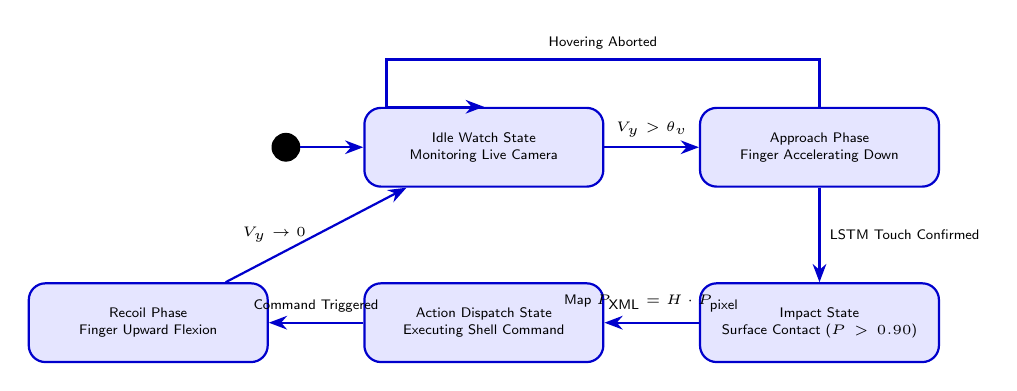
\begin{tikzpicture}[
    state/.style = {rectangle, draw=blue!80!black, fill=blue!10!white, thick, rounded corners=6pt, align=center, font=\sffamily\tiny, text width=2.8cm, minimum height=1.0cm},
    start/.style = {circle, draw=black, fill=black, inner sep=0pt, minimum size=10pt},
    arrow/.style = {draw=blue!80!black, ->, >=Stealth, thick, font=\sffamily\tiny}
]

\node (st) [start] at (0,0) {};
\node (s_idle) [state, right=0.8cm of st] {Idle Watch State\\Monitoring Live Camera};
\node (s_approach) [state, right=1.2cm of s_idle] {Approach Phase\\Finger Accelerating Down};
\node (s_impact) [state, below=1.2cm of s_approach] {Impact State\\Surface Contact ($P > 0.90$)};
\node (s_dispatch) [state, left=1.2cm of s_impact] {Action Dispatch State\\Executing Shell Command};
\node (s_recoil) [state, left=1.2cm of s_dispatch] {Recoil Phase\\Finger Upward Flexion};

\draw [arrow] (st) -- (s_idle);
\draw [arrow] (s_idle) -- node[above]{$V_y > \theta_v$} (s_approach);
\draw [arrow] (s_approach) -- node[right]{LSTM Touch Confirmed} (s_impact);
\draw [arrow] (s_impact) -- node[above]{Map $P_{\text{XML}} = H \cdot P_{\text{pixel}}$} (s_dispatch);
\draw [arrow] (s_dispatch) -- node[above]{Command Triggered} (s_recoil);
\draw [arrow] (s_recoil) -- node[left]{$V_y \to 0$} (s_idle);
\draw [arrow] (s_approach.north) -- ++(0,0.6) -- node[above,font=\sffamily\tiny]{Hovering Aborted} ++(-5.5,0) |- (s_idle.north);

\end{tikzpicture}

\end{document}
